\documentclass{article} 
% \usepackage[vietnamese]{babel}
\usepackage[utf8]{vietnam}
\usepackage{graphicx}
\usepackage{biblatex}
\bibliography{references.bib}

\graphicspath{{images/}}


\title{Báo Cáo về Phân Lớp Dữ Liệu Bằng Danh Sách Luật Bayesian cho Bài Toán Dự đoán Đột Quỵ}
\author{Nguyễn Hữu Lộc - 23C15031}
\date{31/12/2024}

\pagenumbering{arabic}

\begin{document}

\maketitle

\tableofcontents


\section{Giới thiệu sơ lược}
Với sự phát triển vượt trôi của các mô hình Large Language Model (LLM) trong thời gian gần đây, rất nhiều giải pháp đã được nghiên cứu và thử nghiệm nhằm mục đích tăng hiệu quả cho kết quả đầu ra, và giải quyết những vấn đề khó khăn. Đặc biệt quan tâm hơn cả là việc tính minh bạch của các mô hình LLM đang chịu nhiều chỉ trích do sự hình thành ảo giác trong quá trình suy luận, dẫn tới các phương pháp nhằm bổ sung dữ liệu cho mô hình Retrieval-Augmented Generation (RAG) được ra đời. Tuy nhiên các mô hình RAG lại có mặt hạn chế về cơ chế lấy dữ liệu từ các Cơ Sở Dữ Liệu Vector (CSDLV) một cách chưa thực tế và thường phụ thuộc vào cài đặt cố định, thiếu tính linh hoạt. Trong báo cáo này, nhóm sẽ giới thiệu đến một phương pháp mới có tính linh hoạt cao tên là Sel-Reflective Retrieval-Augmented Generation (Self-RAG) nhằm giải quyết vấn đề trên. Self-RAG sử dụng một mô hình tương tự như các mô hình LLM khác nhưng đã được huấn luyện lại cho phép nó có thể tự nhận xét, đánh giá câu trả lời thông qua các Reflection Token, được đưa vào bộ dữ liệu học nhằm mục đích cho phép mô hình tự đánh giá nếu câu trả lời có cần phải có trích dẫn hay không, và liệu trích dẫn hiện tại có phù hợp hay không. Từ đó, có 2 loại Reflection Token là "Retrieval" và "Critique" sẽ được đưa vào huấn luyện để mô hình tự tạo sinh ra, khác biệt so với các mô hình là truy cứu RAG rồi ghép vào prompt, còn Self-RAG sẽ tự tạo sinh ra lúc cần truy cứu. Đây chính là điểm tạo nên sự linh hoạt cho mô hình và giúp giảm chi phí huấn luyện. Chi tiết quy trình này có thể thấy thông qua phần bên phải của Hình \ref{fig:overview_self_rag}.

\begin{figure} 
    \centering
    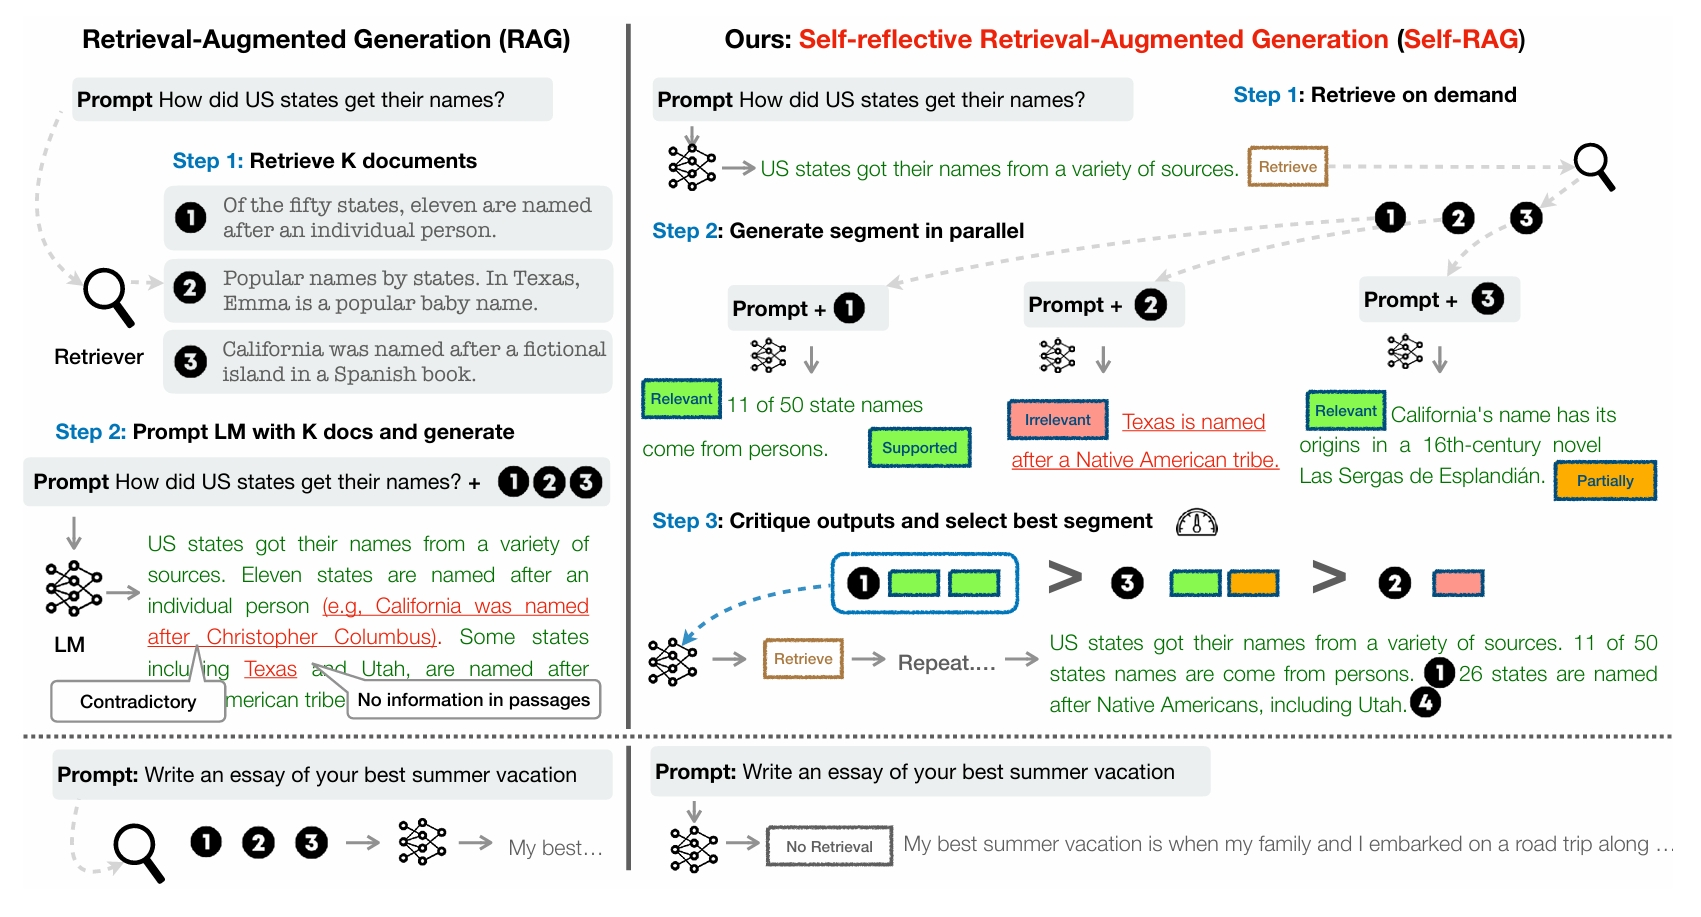
\includegraphics[scale = 0.2]{overview_self_rag.jpeg}
    \caption{Ví dụ về Danh Sách Luật Bayesian}
    \label{fig:overview_self_rag}
\end{figure}

Để chi tiết hơn thì quy trình của Self-RAG có thể được trình bày như sau: 

\begin{enumerate}
    \item Khi tiếp nhận prompts, mô hình đầu tiên sẽ suy luận nếu nó có cần phải truy cứu dữ liệu từ CSDLV hay không. Nếu cần, mô hình sẽ tạo sinh ra Reflection Token "Retrieval" và gọi truy cứu Retriver. 
    \item Kiểm tra xem các dữ liệu truy xuất ra từ CSDLV có tính liên quan với prompts input hay không và tạo sinh ra các câu trả lời tương ứng với từng dữ liệu. 
    \item Tạo sinh các token "Critique" và kiểm tra kết quả trả lời từ mô hình. Tiêu chí sẽ là tính đúng đắn (factuality) và chất lượng câu trả lời (overall quality) rồi cuối cùng mới trả lại câu prompts output.  
\end{enumerate}

Sự khác biệt của Self-RAG so với các mô hình RAG khác là ở chỗ mô hình sẽ tự tạo sinh ra Reflection Token và token này hình thành thông qua huấn luyện đặc biệt với bộ dữ liệu được xử lý bởi một mô hình "critic" khác. Dữ liệu huấn luyện cho Self-RAG đầu tiên sẽ được đưa qua mô hình "critic" để đánh giá, và thay thế các đoạn dữ liệu thành các Reflection Token "Retrieval" và "Critique" tương ứng, từ đó tạo nên bộ dữ liệu huấn luyện có sẵn những token này. Từ đó, dữ liệu này sẽ được đưa vào huấn luyện, cho phép Self-RAG có thể tự tạo ra những yêu cầu đánh giá và truy vấn theo nhu cầu. Điều này giúp tiết kiệm chi phí thay vì dùng 2 mô hình song song, 1 để tạo sinh câu trả lời và 1 để đánh giá, khi đưa vào thực tế như một vài phương pháp lồng ghép việc đánh giá kết quả từ truy vấn khác như mô hình Adaptive RAG \cite{jeong2024adaptive}. 


\section{Các công trình liên quan}

\section{Self-RAG: Học cách tìm nguồn, tạo sinh và đánh giá}

\subsection{Sơ lược bài toán và phương pháp}

\subsection{Huấn luyện Self-RAG}

\subsubsection{Huấn luyện phần đánh giá}

\subsubsection{Huấn luyện phần tạo sinh}

\subsubsection{Suy Luận}

\section{Thí nghiệm}

\subsection{Bài toán và dữ liệu}

\subsection{Cài đặt thí nghiệm}

\section{Kết quả và Phân tích}

\subsection{Kết quả}

\subsection{Phân tích}

\section{Kết luận}


\printbibliography

\end{document}